\documentclass[oneside]{VUMIFPSkursinis}
\usepackage{algorithmicx}
\usepackage{algorithm}
\usepackage{algpseudocode}
\usepackage{amsfonts}
\usepackage{float}
\usepackage{amsmath}
\usepackage{bm}
\usepackage{caption}
\usepackage{color}
\usepackage{float}
\usepackage{graphicx}
\usepackage{listings}
\usepackage{subfig}
\usepackage{tabularx}
\usepackage{wrapfig}
\newcolumntype{P}[1]{>{\centering\arraybackslash}p{#1}}
\usepackage[%  
    colorlinks=true,
    linkcolor=black
]{hyperref}
\university{Vilniaus universitetas}
\faculty{Matematikos ir informatikos fakultetas}
\department{Programų sistemų katedra}
\papertype{Laboratorinis darbas III}
\title{Automatinė ūkio valdymo sistema}
\titleineng{Automatic Farm Management System}
\status{2 kurso 3 grupės studentai}
\author{Matas Savickis}
\secondauthor{Justas Tvarijonas}  
\thirdauthor{Greta Pyrantaitė}   
\fourthauthor{Rytautas Kvašinskas}
\supervisor{Karolis Petrauskas, Doc., Dr.}
\date{Vilnius – \the\year}


\bibliography{bibliografija}

\begin{document}
\maketitle
\centering
\tableofcontents


\section{Įvadas}
Šia dokumente pateikiama Automatinės ūkio valdymo sistemos(toliau Auto ūkis) verslo analizę. Autoūkis yra sistema suteikianti vartotojui galimybę automatizuoti žemės ūkio valdymą. Sistema suteikia galimybę žemės ūkio techniką: pirkti, parduoti, automatikšai valdyti. Mūsų sistema galima kontroliuoti žemės plotus, juos laistyti bei sekti dirvos parametrus. Vartotojui taip pat suteikiama galimybė samdyti bei atelisti darbuotojus, išrašinėti sąskaitas bei užsiimti kitaip buhalteriniais veiksmais. Tarp panaudojimo galimybių yra ir gyvūnų sekimas realiu laiku, jų informacijos surašymas, bei automatinis gyvūnų maitinimas. Ūkininkas taip pat gali registruoti savo derlių, stebėti rinko ir planuoti būsimą pelną. Visa sistema yra moduli kas reiškia, kad sistema yra išskirstytą į keletą atskirų fragmentų ir jų visų potencialiam pirkėjui įsigyti nereikia. Sistemos kūrėjai yra atsakingi už sistemos įdiegimą, bet ne palaikymą. Sistemą turi palaikyti pats pirkėjas arba samdyti mūsų pačių apmokytus technikus.
\section{Verslo proceso aprašas}
\section{Išorinė analizė}
	\subsection{Verslo įeiga/išeiga}
	\subsection{Tiekimo grandinė}
	\begin{itemize}
\item Diagramoje (1 pav.) pavaizduoti pagrindiniai tiekėjai bei pirkėjai, su kuriais bendrauja mūsų nagrinėjamos srities atstovai.
		\begin{figure}[H]
		\centering	
	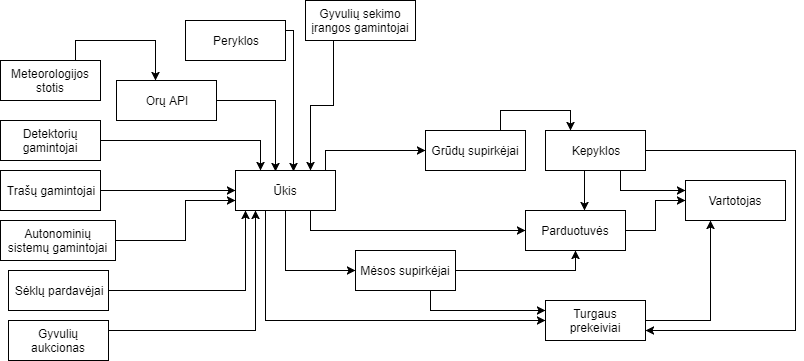
\includegraphics[width=18cm,height=20cm,keepaspectratio]{supplyChain.png}
	\caption{Tiekimo grandinė}
	\label{fig:supplyChain}
\end{figure}
\end{itemize}
\subsubsection{Pirkėjų apibrėžimas}
Kaip pagrindinius ūkio sukuriamos produkcijos pirkėjus galime įvardinti eilinius žmones, kadangi praktiškai visa ūkio produkcija suvartojama maisto pavidalu. Žinoma dauguma žmonių šią produkciją perka ne tiesiai iš ūkininkų, o iš perpardavinėtojų ar perdirbėjų, kurie ūkio teikiamą produkciją paverčia į jau paruoštą vartoti produktą. Taigi nors iš pirmo žvilgsnio atrodo, kad ūkio produkcijos pirkėjai yra perpardavinėtojai ir perdirbėjai, tačiau tikrieji pirkėjai yra tie, kurie perka galutinį produktą, kadangi į visas darbas yra orientuotas į juos.
\subsubsection{Pirkėjų poreikiai}
Šioje diagramoje matome, kad ūkio atstovai savo produkciją paskirsto 4 keliais, tačiau juos galime padalinti į dvi dalis, ūkio tiekiama produkcija turgaus prekeiviams sudaro labai mažą dalį visos produkcijos, kadangi šią sritį dažniausiai pasirenka tie ūkininkai, kurie turi mažesnį kiekį produkcijos ir jiems mažesnių kiekių pardavinėjimas nesukelia jokių problemų, didesni ūkiai priklausomai nuo jų sukuriamo produkto paprastai renkasi parduotuves bei mėsos arba grūdų supirkėjus, kadangi jie pajėgus produkciją supirkti labai dideliais kiekis taip palengvindami ūkio produkcijos administravimą. Iš šių subjektų, kurie bendrauja su ūkio kokybei didžiausius reikalavimus kelia turgaus prekeiviai bei parduotuvės atstovai, kadangi jie tiesiogiai bendrauja su vartotojais, o vartotojai visada tikisi aukščiausios kokybės produkcijos. O mėsos ir grūdų supirkėjai paprastai užsiima masiniu produkcijos perdirbimu, ko pasekoje šiek tiek prastesnės kokybės produktai jiems nesudaro didelių kliučių pateikti vartotojui tinkamos kokybės produktą.
\subsubsection{Derybinės galimybės su tiekėjais}
Panašiai kaip ir pirkėjus, taip ir tiekėjus galime suskirstyti į dvi pagrindines grupes. Tokie tiekėjai, kaip trašų gamintojai, sėklų pardavinėtojai, meteorologai ar peryklos bei gyvulių pardavėjai neturi didelės derybinės galios, kadangi panašią ar netgi tokią pačią pasiūlą teikiančių tiekėjų yra pakankamai didelis kiekis, todėl patys ūkio atstovai gali išsirinkti jiems geriausius pasiūlymus ir daugelio pasirinkimų. Tačiau visai kita situacija su kitais tiekėjais, tokie tiekėjai kaip sekimo įrangos gamintojai dar galbūt ir neturi labai didelės derybinės galios, tačiau like tiekėjai gali teikti savo reikalavimus, kadangi ūkio atstovai nelabai turi kitų alternatyvų pagrūdintiniems šių tiekimo šakų atstovams, tokia tiekimo šaka kaip autonominių sistemų gamintojai turi maždaug 2-3 didesnius ir klientus patrauklesnius atstovus ir kiekvienas iš jų orientuojasi į šiek tiek kitą pusę, ko pasekoje ūkio atstovai turi rinktis iš daugiausiai 2 tiekėjų, kurių kiekvienas neturi poreikio visomis išgalėmis siekti sutarties nuleidžiant kainas, kadangi jie tiesiog neturi rimtos konkurencijos.
	\subsection{Efektyvumas}
	\subsection{Grėsmės/galimybės}
\section{Vidinė dalykinės srities analizė}
	\subsection{Veiklos principai}
	\subsection{Rodikliai}
\section{Analizės rezultatai, apibendrinimas}
	\subsection{Stiprybės}
	\subsection{Silpnybės}
	\subsection{Galimybės}
	\subsection{Pavojai}
\section{Vizija, misija}
\section{Strateginiai tikslai}
\section{Sistemos naudojimo scenarijus}
\section{Sistemos įgyvendinimo planas}
\section{Įgyvendinamumo analizė}
	\subsection{Operacinė analizė}
	\subsection{Techninė analizė}
	\subsection{Ekonominio įgyvendinamumo analizė}
	\subsection{Teisinė analizė}
\section{Išvados}
\section{Žodynas}

\end{document}